%!TEX program = xelatex
\documentclass[a4paper, 11pt]{article} % Font size (can be 10pt, 11pt or 12pt) and paper size (remove a4paper for US letter paper)

%\documentclass{article}
%\usepackage[protrusion=true,expansion=true]{microtype} % Better typography
\usepackage{graphicx} % Required for including pictures
\usepackage{wrapfig} % Allows in-line images
\usepackage{ctex}

\usepackage{mathpazo} % Use the Palatino font
\usepackage[T1]{fontenc} % Required for accented characters
\usepackage{fontspec}
\usepackage{xunicode}
\usepackage{xltxtra} 
\usepackage{amsmath}
\usepackage{geometry}
\usepackage[colorlinks,linkcolor=black]{hyperref}
\geometry{a4paper,scale=0.7}
\linespread{1.05} % Change line spacing here, Palatino benefits from a slight increase by default
%\linespread{0.5}
\makeatletter
\renewcommand\@biblabel[1]{\textbf{#1.}} % Change the square brackets for each bibliography item from '[1]' to '1.'
\renewcommand{\@listI}{\itemsep=0pt} % Reduce the space between items in the itemize and enumerate environments and the bibliography

\renewcommand{\maketitle}{ % Customize the title - do not edit title and author name here, see the TITLE block below

\begin{flushright} % Right align
{\LARGE\@title} % Increase the font size of the title

\vspace{50pt} % Some vertical space between the title and author name

{\large\@author} % Author name
\\\@date % Date

\vspace{10pt} % Some vertical space between the author block and abstract
\end{flushright}
}

%----------------------------------------------------------------------------------------
%	TITLE
%----------------------------------------------------------------------------------------

\title{\textbf{Introduction to Probability}\\ % Title
Markov Chain 2} % Subtitle

\author{\textsc{Yan Hao} % Author
\\{\textit{ACM Class,2016}}} % Institution

\date{\today} % Date

%----------------------------------------------------------------------------------------

\begin{document}

\maketitle % Print the title section

%----------------------------------------------------------------------------------------
%	ABSTRACT AND KEYWORDS
%----------------------------------------------------------------------------------------

%\renewcommand{\abstractname}{Summary} % Uncomment to change the name of the abstract to something else

%\tableofcontents
\begin{abstract}
该节主要对马尔可夫链做出了进一步的介绍。

第一部分讨论了函数在马尔可夫链上的作用,即马尔可夫链经函数作用后是否仍是马尔可夫链。首先给出了两个马尔可夫链的例子,这两个例子正好可以通过特定函数作用由一个转化为另一个。接着,给出了一个马尔可夫链映射后不再是马尔可夫链的例子。最后,给出了一个马尔可夫链经映射后仍为马尔可夫链的充分条件。

第二部分给出了两个定理。第一个定理为马尔可夫链不可约等价于强连通。第二个定理为,每一个马尔可夫链都有且只有一个稳定分布。随后分别从三个方面证明了第二个定理,即矩阵证明,不动点证明,概率论证明。
\end{abstract}
\vspace{10pt} % Some vertical space between the abstract and first section

\tableofcontents
%----------------------------------------------------------------------------------------
%	ESSAY BODY
%----------------------------------------------------------------------------------------
\newpage
\section{Function on Markov Chain}
\subsection{Problem}
\begin{small}
%\begin{itemize}
%\item
已知有马尔可夫链$M_1$
$$
M_1=\left(X_0,X_1,X_3,...,X_n\right)
$$

若有映射f作用在$M_1$上,得到$M_2$
$$
M_2=\left(f_{(X_1)},f_{(X_2)},f_{(X_3)},...,f_{(X_n)}\right)
$$

问:在f满足什么条件的情况下$M_2$是马尔可夫链?在什么情况下$M_2$不是马尔可夫链?
%\item
\end{small}
\subsection{Examples of Markov Chain}
\subsubsection{Ehrenfest urn}
\begin{figure}[h]
    	\centering
    	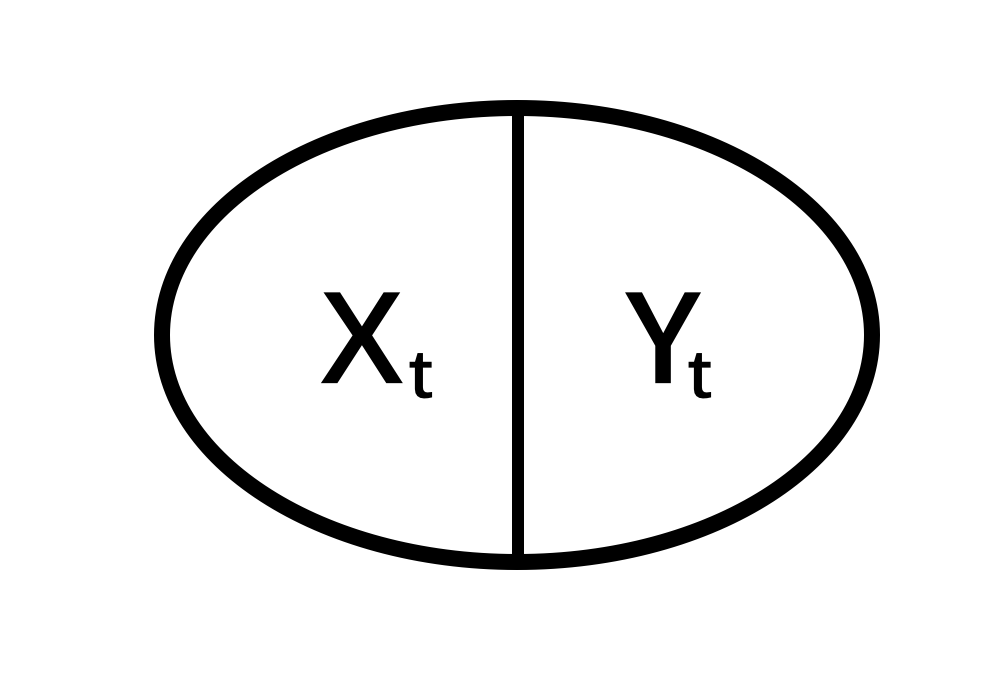
\includegraphics[width=0.5\textwidth]{figures//figure1}
    	\caption{篮球分割问题}
\end{figure}
\begin{small}
如图1所示,假设共有n个篮球,t时刻在X篮筐里有$X_t$个篮球,在Y篮筐里有$Y_t$个篮球.每一时刻随机地从这n个篮球里选择一个,放入另一个篮筐里.
\begin{itemize}
	\item 状态变化由$(1)$描述
    \begin{equation}  
     \left\{  
             \begin{array}{lr}  
             X_t+Y_t=n &  \\  
             X_t=X_t+1, Y_t=Y_t-1\ /\ X_t=X_t-1,Y_t=Y_t+1 & 
            \end{array}  
    \right.  
    \end{equation}  
	
	\item 状况集表示:$(0,1,2,3,...,n)$, 即用X筐或Y筐中篮球的数量描述特定状态.
\end{itemize}
\end{small}
\newpage
\subsubsection{Hypercube}
\begin{small}
\begin{figure}[h]
    	\centering
    	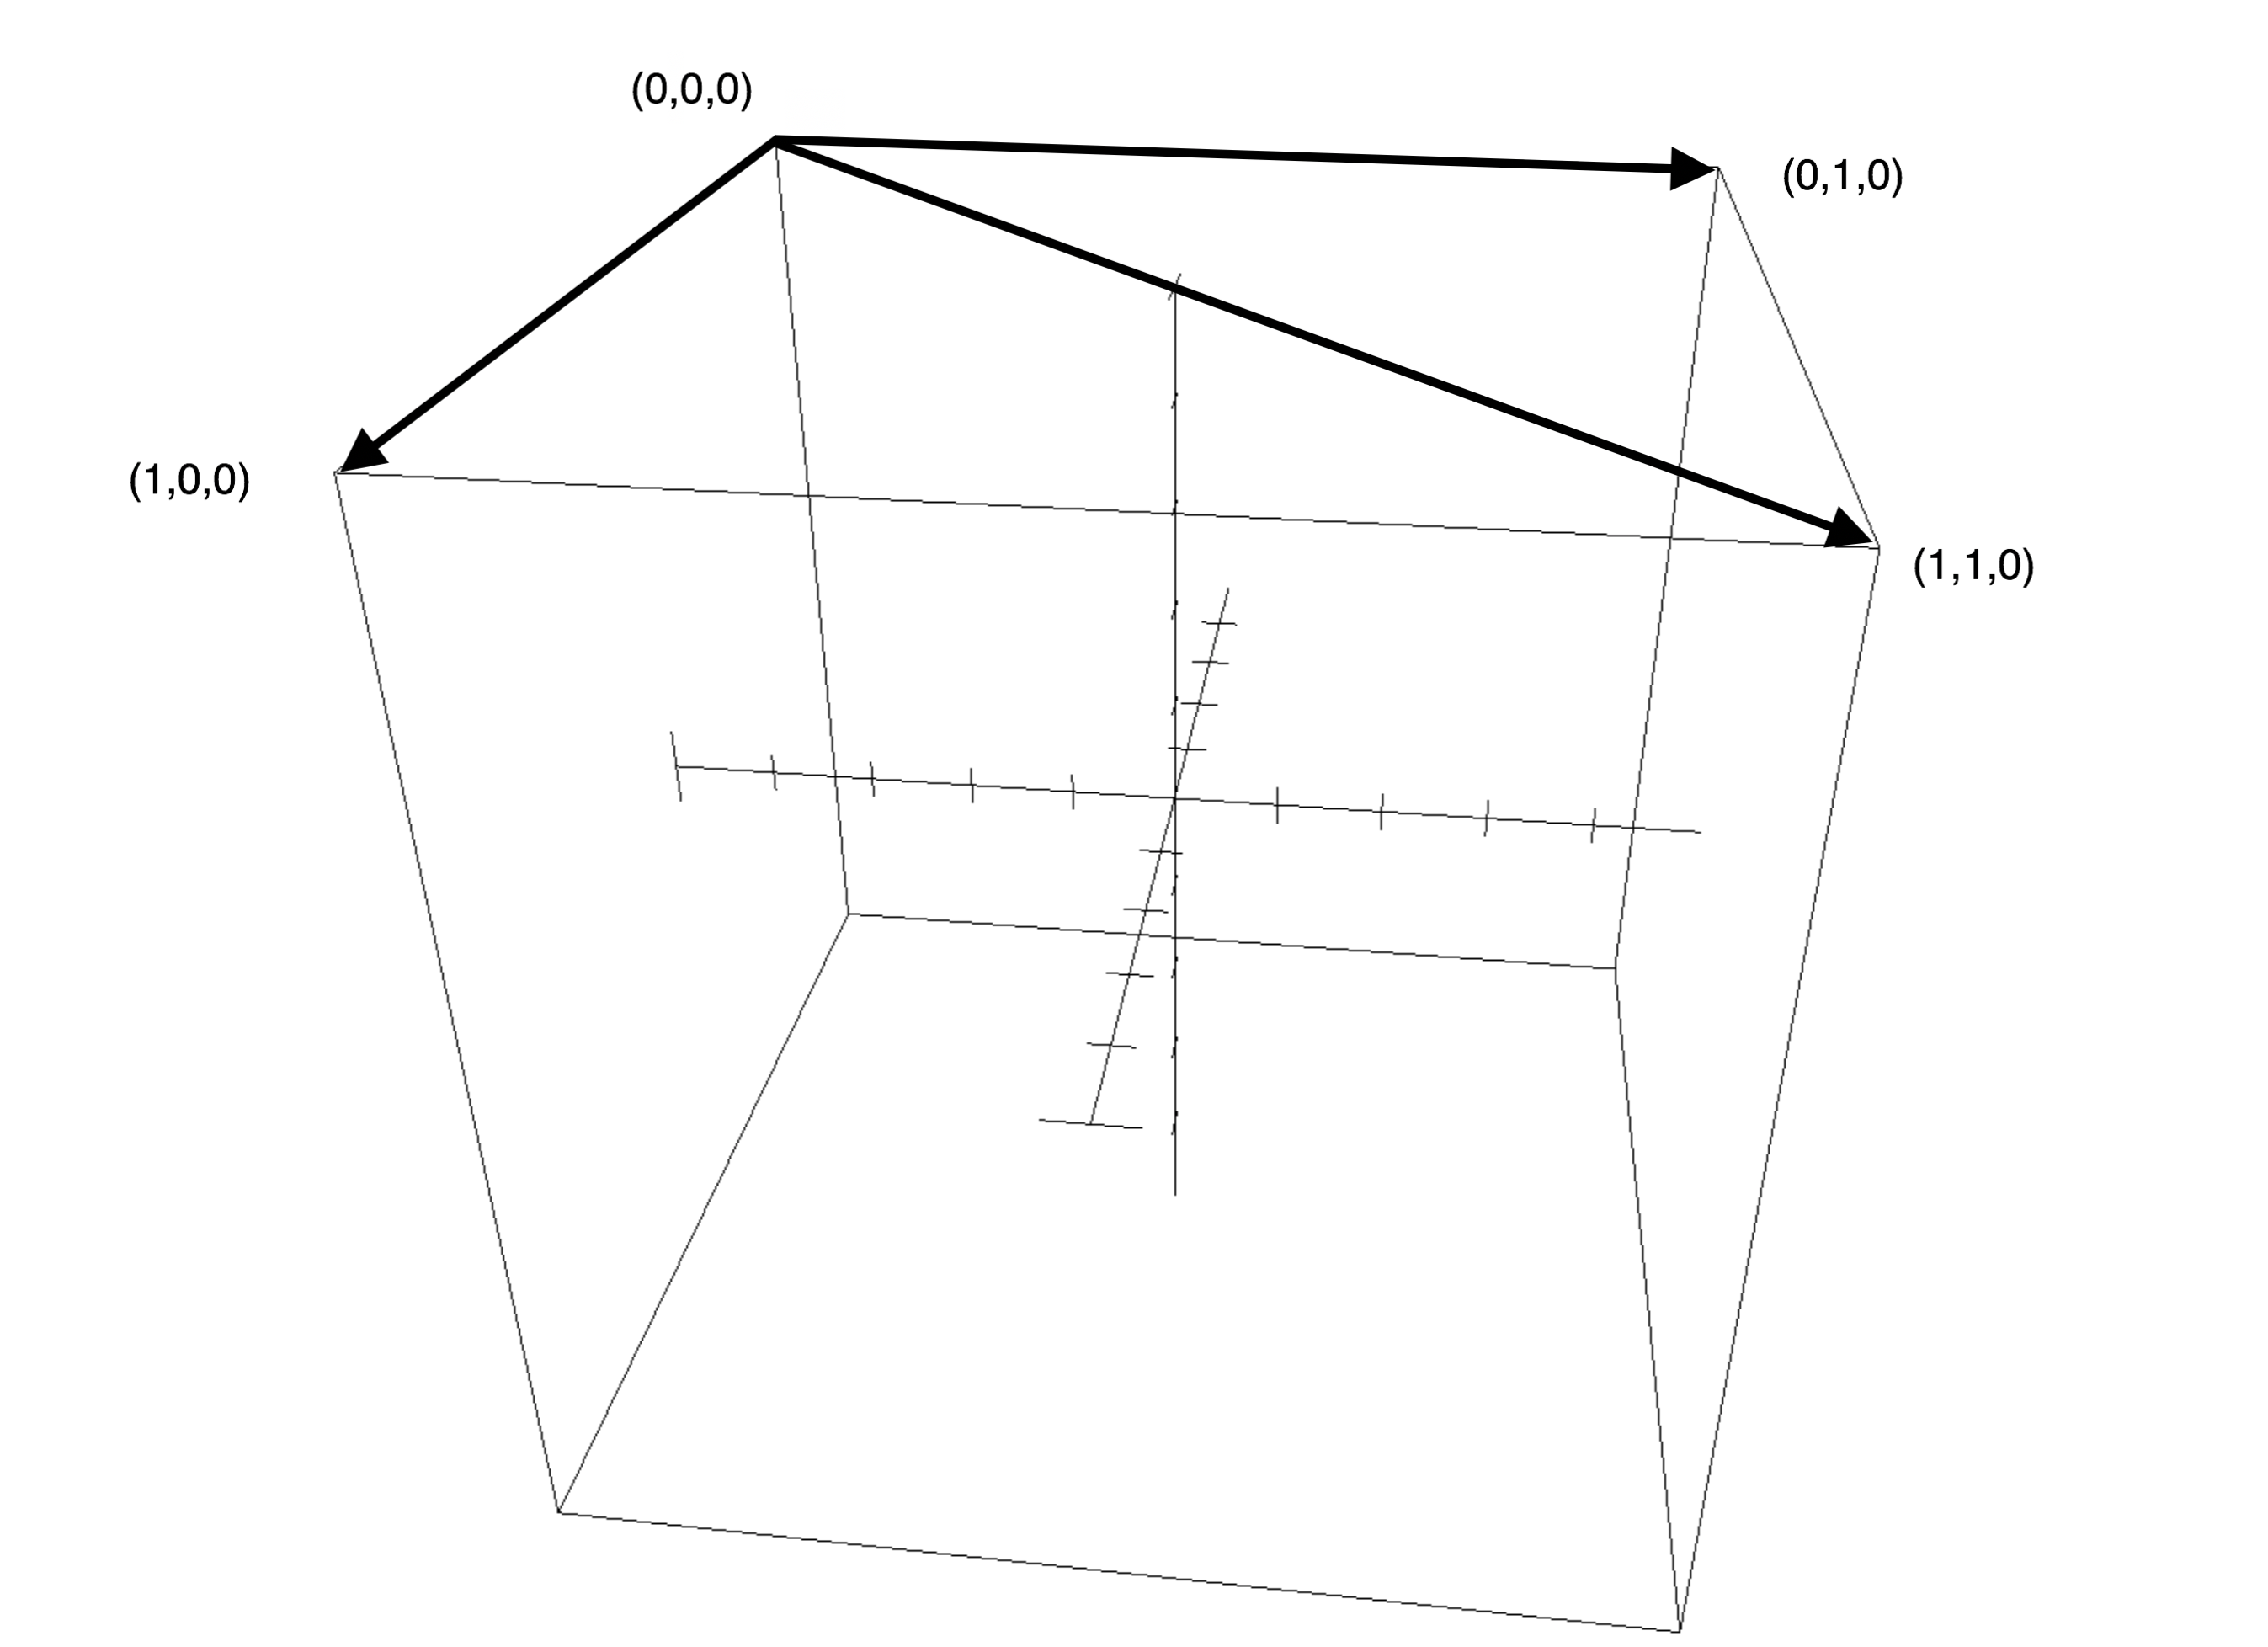
\includegraphics[width=0.99\textwidth]{figures//figure3}
    	\caption{立方体上的随机游走}
\end{figure}
\begin{itemize}
	\item 假设立方体的每一个顶点上都有若干小球,随机地沿着边游走(该模型用立方体上的随机游走表示马尔可夫链从一个状态到下一个状态)
	\item 每一个顶点表示一个状态,共$2^3$个状态
	\item 每条边的边权表示从一点到另一点的可能性大小,即
	      \begin{equation}  
           P_{(i,j)}\left\{  
             \begin{array}{lr}  
              \frac{1}{3} \  (i\ is\ adjacent\ to\ j)&  \\  
             0 \  (i\ is\ not\ adjacent\ to\ j) & 
            \end{array}  
         \right.  
         \end{equation} 
	\item 该分布是可逆的,即
	$$\Pi _iP_{ij}=\Pi _jP_{ji}$$
	因此立方体总的质量分布没有改变,可以认为是平稳分布,即
	$$\Pi P= \Pi $$
	\item 推广:若度数为n,则可表示$2^n$个状态
\end{itemize}
\end{small}


\subsection{Analysis}
\begin{small}
\subsubsection{Examples of $f_{(M)}$}
\begin{itemize}
	\item $M_1$经过映射后得到的$M_2$仍是马尔可夫链:
	\\ 将1.2.2中Hypercube中的状态映射到1.2.1中Ehrenfest urn的状态中.
	$$\mbox{f的作用:若向量有n个维度是1,则将该向量映射为n}$$
	$$(0,0,0,...,0)\rightarrow0$$
	\begin{equation}  
           \left\{  
             \begin{array}{lr}  
              (1,0,0,..,0)&  \\  
             (0,1,0,..,0) &  \\ 
             ......& \\
             (0,0,0,..,1)
            \end{array}  
         \right.  
         \rightarrow 1
      \end{equation}
      $$\mbox{......}$$
       $$\mbox{依此类推,则f将一个马尔可夫链映射为了另一个马尔可夫链}$$

	\item $M_1$经过映射后得到的$M_2$不再是马尔可夫链:
	%$$\mbox{f:}$$
	\begin{figure}[h]
    	\centering
    	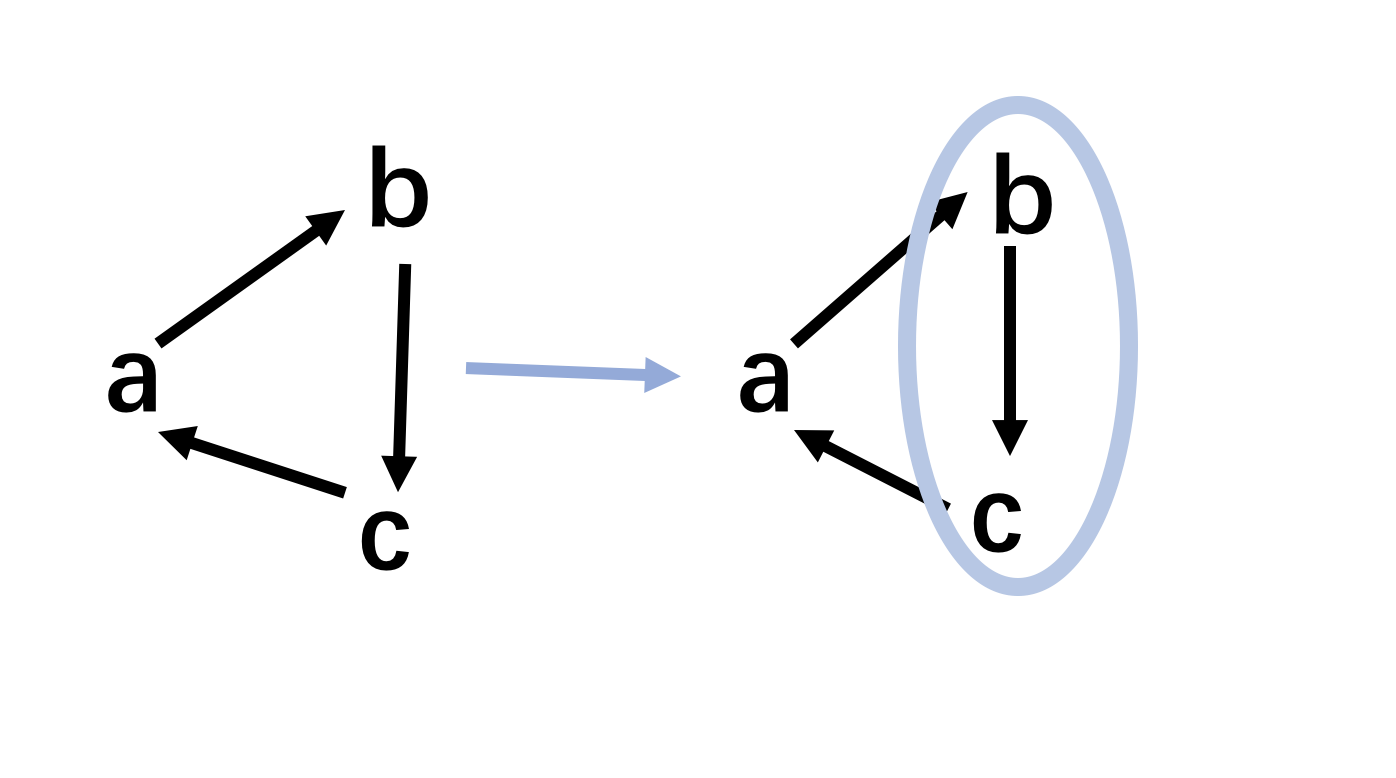
\includegraphics[width=0.8\textwidth]{figures//figure2}
    	%\caption{马尔可夫链的映射}
    \end{figure}
    \begin{enumerate}
    	\item 映射前:$a\rightarrow b,b\rightarrow c,c\rightarrow a$
    	下一个状态只与当前状态有关,因此是马尔可夫链
    	\item 映射后,状态集变为两个,即$(a,\left\{b,c\right\})$
    	设t时刻状态$S_t$为${b,c}$,则
    	$$
    	 S_{t-1}=\left\{b,c\right\}\rightarrow S_{t+1}=a
    	$$
    	$$
         S_{t-1}=a\rightarrow S_{t+1}=\left\{b,c\right\}
    	$$

    \end{enumerate}
    $$\mbox{下一个状态不但与当前状态有关,还与上一个状态有关,因此不是马尔可夫链}$$
    $$\mbox{f将一个马尔可夫链映射为了一个非马尔可夫链}$$
\end{itemize}
\subsubsection{sufficient condition}
\begin{itemize}
	\item 
	$$
	M_1 \xrightarrow{f} M_2 \Longleftrightarrow x\xrightarrow{f} [x] 
	$$
	即f作用在$M_1$上等价于把原本的数据集划分为等价类
	\item lemma 1\\
	If $P_{(x,[y])}=P_{(x^{'},[y])}$ is true whenever $[x]=[x^{'}]$, then $([x_1],[x_2],[x_3],...,[x_n])$ is Markov Chain.
	\item 
	若f不满足lemma 1的条件,$M_2$是否有可能是马尔可夫链?试给出分析
\end{itemize}


\end{small}

\begin{small}
\section{Theorem}
\subsection{Irreducible and Strongly Connected}
前提:马尔可夫链可以表示为n阶实数方阵A,其中$A(i,j)=1$表示由状态i可以到达状态j,$A(i,j)=0$表示由状态i无法到达状态j.

Theorem1: 矩阵A是不可约的当且仅当与A对应的有向图S(A)是强连通的.

proof:
\begin{itemize}
	\item 强连通的概念:一个有向图中任意两点v1、v2间存在v1到v2的路径及v2到v1的路径.
	\item 不可约的概念:对于矩阵$A=R^{n*n}$,如果存在置换矩阵P,使得
	$$
	  PAP^{T}=\begin{pmatrix} B & C \\ 0 & D \end{pmatrix}\quad
	$$
	则矩阵A可约,否则A不可约
	\item lemma2:\\
	矩阵$A_1$是有向图D的邻接矩阵。矩阵$A_2$
也是D的邻接矩阵的充分必要条件是存在置换阵
P,使得$A_2=PA_1P-1$
    \item 由以上三条可知,经置换操作后的矩阵$A_2$与矩阵$A_1$表示的是同一个有向图。因此若某一矩阵不可约,则其形式一定为
    $$
	  A=\begin{pmatrix} B & C \\ E & D \end{pmatrix}\quad
	$$
	即该矩阵的四个模块之间彼此连通
\end{itemize}
\subsection{Stational Distribution}
Theorem:对于所有有限状态的马尔可夫链,存在且仅存在一个平稳状态$\pi$(stational distribution)

稳定分布$\pi$是一个(行)向量,它的元素都非负且和为1,不随施加P操作而改变,定义为
$$
  \pi P= \pi
$$

\subsubsection{Proof 1}
矩阵法证明

对于一个离散状态空间,对于k步转移后的状态,可以对转移矩阵求 k次幂来求得。就是说,如果P是一步转移矩阵,$P^k$即为k步转移后的转移矩阵。如果转移矩阵P不可约,并且是非周期的,则$P^k$收敛到一个每一列都是不同的平稳分布$\pi ^{*}$,并且
$$
 \lim_{k\rightarrow \infty} P^k=\pi ^{*}
$$
且独立于初始分布\\
以上由Perron–Frobenius theorem所指出,
参考如下\\
\url{https://en.wikipedia.org/wiki/Perron%E2%80%93Frobenius_theorem}

\subsubsection{Proof 2}
不动点法证明

\subsubsection{Proof 3}
概率论方法证明
\begin{itemize}
	\item 对于所有状态x,定义x的hitting time:
	$$
	  \tau_x=\min\left\{t\geq0, x_t=x\right\}
	$$
	$$
	  \tau_x^{+}=\min\left\{t\geq1, x_t=x\right\}
	$$
	\item lemma 3:$\  $For any state x,y of an irreducible chain, $E_x\left\{\tau_y^{+}\right\}<\infty$\\
	Proof of lemma 3:
	$$\exists \varepsilon > 0\ and\ r>0,such\ that$$
	$$\forall z,w \in \Omega,\ \exists j\leq r$$
	$$
	 s.t.\ P_{(z,w)}^j>\varepsilon
	$$ 
	利用irreducible的定义\\
	$$
	P_x\left\{\tau_y^{+}>kr\right\}<(1-\varepsilon)P_x\left\{\tau_y^{+}>(k-1)r\right\}
	$$
	$$
	\mbox{以此类推......}
	$$
	$$
	 P_x\left\{\tau_y^{+}>kr\right\}<(1-\varepsilon)^k
	$$
     由于
     $$
     \sum _{t\geq 0}tP_x\left\{\tau_y^{+}=t\right\}=\sum _{t\geq 0}P_x\left\{\tau_y^{+}>t\right\}
     $$
     因此
     \begin{align*}
     E_x\left\{\tau_y^{+}\right\}&=\sum _{t\geq 0}tP_x\left\{\tau_y^{+}=t\right\}\\
     &=\sum _{t\geq 0}P_x\left\{\tau_y^{+}>t\right\}\\
     &\leq \sum _{k\geq 0}rP_x\left\{\tau_y^{+}>kr\right\}\\
     &<r\sum _{k\geq 0}(1-\varepsilon)^k\\
     &=\frac{r}{\varepsilon}\\
     &<\infty
     \end{align*}
     $$
     \mbox{因此,}E_x\left\{\tau_y^{+}\right\}<\infty \mbox{成立}
     $$
	\item proof:\\
	欲说明$\pi(x)=\frac{1}{E_x\left\{\tau_x^{+}\right\}}\ $s.t.$\ \pi P=\pi$且$\sum _{x\in \Omega}\pi(x)=1$
	\begin{enumerate}
		\item
    $$
    \forall z \in \Omega\  \widetilde{\pi}(y)=E_z(number\ of\ visit\ to\ y\ before\ returning\ to\ z)\leq E_z\left\{\tau_z^{+}\right\}
    $$
    $$
    \mbox{According to lemma 3, $E_z\left\{\tau_z^{+}\right\}$ is well defined}
    $$
    $$
     \widetilde{\pi}(z)=1
    $$
    \item
     \begin{align*}
    \sum _{x\in \Omega}\widetilde{\pi}(x)P(x,y)
     &=\sum_{x\in \Omega}\sum_{t\geq0}P_z(X_t=x,\tau_z^{+}>t)P(x,y)\\
     &=\sum_{t\geq0}\sum_{x\in \Omega}P_z(X_t=x,\tau_z^{+}>t)P(x,y)\\
     &=\sum_{t\geq0}\sum_{x\in \Omega}P_z(X_t=x,X_{t+1}=y,\tau_z^{+}>t)\\
     &=\sum_{t\geq0}P_z(X_{t+1}=y,\tau_z^{+}>t)\\
      &=\sum_{t\geq1}P_z(X_{t+1}=y,\tau_z^{+}\geq t)\\
      &=\sum_{t\geq1}[P_z(X_{t+1}=y,\tau_z^{+}=t)+P_z(X_{t+1}=y,\tau_z^{+}>t)]\\
      &=\sum_{t\geq1}P_z(X_{t+1}=y,\tau_z^{+}= t)+\widetilde{\pi}(y)-P_z(X_{0}=y,\tau_z^{+}>0)\\
      &=\widetilde{\pi}(y)
     \end{align*}
     $$
     \mbox{因此}\Longrightarrow \widetilde{\pi}P=\widetilde{\pi}
     $$
     \item
     取$z=x$
     $$
     \pi = \frac{\widetilde{\pi}^{(z)}}{E_z\left\{\tau_z^{+}\right\}}\Longrightarrow \pi(x) = \frac{\widetilde{\pi}^{(x)}(x)}{E_x\left\{\tau_x^{+}\right\}}=\frac{1}{E_x\left\{\tau_x^{+}\right\}}
     $$
 \end{enumerate}
\end{itemize}


\section{Contact Me}
Email:$\  $honeyhaoyan@sjtu.edu.cn

以上笔记可能有很多缺漏,如有问题,请及时联系我,谢谢!

\end{small}
%----------------------------------------------------------------------------------------
%	BIBLIOGRAPHY
%----------------------------------------------------------------------------------------

%\bibliographystyle{unsrt}

%\bibliography{sample}

%----------------------------------------------------------------------------------------

\end{document}